\chapter{Model Predictive Control Setup}
\label{chapter:MPC}
This chapter presents the setup and creation of the MPC controller, and investigates the performance of the resulting controller on the greenhouse environment. Moreover, the effect of the prediction horizon is investigated on both nominal and stochastic conditions. The works in this chapter is similar to what is presented in \cite{boersmaRobustSamplebasedModel2022} and \cite{morcegoReinforcementLearningModel2023}. However, direct comparisons are not possible. \cite{boersmaRobustSamplebasedModel2022} develops to create a robust sample based controller, while this chapter will focus on constructing a conventional Model Predictive Controller (MPC). This is done to examine the effects of uncertainty on this controller and later asses whether the integration of RL can mitigate these effects. In \cite{morcegoReinforcementLearningModel2023}, such an MPC controller is developed. However, it does not provide specific weather data. Finally the optimization goal used in this thesis differs from that in both papers. However, a qualitative comparison may be done.




\section{Greenhouse MPC problem formulation}
In order to directly compare to RL and to the RL-MPC controller, it is important that the optimization goal is equivalent. As discussed in \autoref{ssection:optimization-goal}, it is desired to optimize the economic benefit of the greenhouse environment. Similarly to \autoref{section:env-description}, the optimization goal of the MPC is done to ensure that the sum of stage costs are equal to the actual economic benefit of the system. As such the following optimization goal is solved at every time step:

\begin{subequations} \label{eq:mpc_ocp}
	\begin{align}
		\min_{u(k),x(k)} & \sum_{k = k_0}^{k_0 + N_p-1} {l(u(k), y(k))} \\
		\text{s.t.} \quad & x(k+1) = f(x(k), u(k), d(k), p),  \label{eq:constraint-1} \\
		& y(k) = g(x(k+1), p), \label{eq:constraint-dynamics} \\
		& -\delta u \leq u(k) - u(k-1) \leq \delta u, \label{eq:constraint-delta-u} \\
		& u_{\min} \leq u(k) \leq u_{\max}, \label{eq:constraint-u-limits}\\
		& x(k_0) = x_{k_0}. \label{eq:constraint-initial}
	\end{align}
\end{subequations}

To ensure that the optimization goal is exactly the same as the Rl reward function (\autoref{section:env-description}), the cost function $V(u(k),y(k))$ becomes:

\begin{equation} \label{eq:mpc_cost_function}
	\begin{aligned}
		l(u(k),y(k)) & = - \kappa_1 (y(k) - y(k-1)) + \sum_{j=2}^4 {\kappa_j u_{j-1}} + \sum_{i = 1}^4 s_i(k) \\
		\text{where} & \quad s_i(k) \geq 0, \\
		& s_1(k) \geq c_{p_{C02}} \cdot (y_2^{min} - y_2(k)), \\ 
		& s_2(k) \geq c_{p_{C02}} \cdot (y_2(k) + y_2^{max}), \\ 
		& s_3(k) \geq c_{p_{T_{lb}}} \cdot (y_3^{min} - y_3(k)), \\ 
		& s_4(k) \geq c_{p_{T_{ub}}} \cdot (y_3(k) + y_3^{max}), \\ 
		& s_5(k) \geq c_{p_{H}} \cdot (y_4^{min} - y_4(k)), \\ 
		& s_6(k) \geq c_{p_{H}} \cdot (y_4(k) + y_4^{max}), \\
	\end{aligned}	
\end{equation}

where the slack variables are introduced in order to accommodate the output constraint in equation \autoref{eq:mpc_ocp}, resulting in an optimization problem equivalent to that of RL. The penalty constants $c_{p_{C02}},c_{p_{T_{lb}}},c_{p_{T_{ub}}},c_{p_{H}}$ are the same as what is used in the Rl problem formulation and given in \autoref{tab:pen-constants}.

\paragraph{Experimental Setup} Furthermore, the experimental setup is identical to what is used in \autoref{section:experimental-setup} with the exception of normalizing observations. The performance metrics are the sum of the stage costs during the simulation period, which is equivalent to the EPI minus the sum of the state violations. For the stochastic environment, the performance metric is calculated by taking the average of the sum of stage costs over 30 simulation periods, as well as considering the variance of the resulting stage costs. In the case of stochasticity, the MPC algorithm still solves the optimization problem defined by equation \autoref{eq:mpc_ocp} using the nominal system parameters. However, it is only during the system evolution that the uncertainty in parameters is taken into account. 

Finally, to increase the computational time and feasibility of the MPC solver, the solver is warm-started with the previous solution to reduce the number of iterations required to reach the optimal solution  \footnote{The solution to the OCP is heavily reliant on initial guesses due to the non-linearity nature of the problem, lagrangian multipliers from the previous solutions were also reused to mitigate instability in the solver. These instabilities are especially prevalent in longer prediction horizons}. The computational time of computing the optimal control actions will also be examined for each prediction horizon. These performance metrics are given for all prediction horizons. Finally, The MPC framework is built using the open source software Casadi \textbf{ref XXX} and the non-linear solver IPOPT \textbf{ref xxx} in python. 

\section{Deterministic Results}
Simulations are conducted for every prediction horizon $N_p$.The prediction horizons to be tested will include time intervals of 1 hour, 2 hours, 3 hours, 4 hours, 5 hours, and 6 hours. Results include the final cumulative reward and the average time required to solve \autoref{eq:mpc_ocp} for each prediction horizon.

\begin{figure}[H]
	\centering
	\begin{subfigure}[b]{0.49\textwidth}
		\centering
		\includegraphics[width=\textwidth]{figures/mpc_nominal_perf.eps}
		\caption{Final cumulative reward of MPC on nominal conditions}
		\label{fig:mpc_nominal_perf}
	\end{subfigure}
	\hfill
	\begin{subfigure}[b]{0.49\textwidth}
		\centering
		\includegraphics[width=\textwidth]{figures/mpc_nominal_compt_time.eps}
		\caption{Computational Time of MPC control actions}
		\label{fig:mpc_nominal_comp_time}
	\end{subfigure}
	\caption{MPC Performance Metrics}
	\label{fig:mpc_metrics_nominal}
\end{figure}

\autoref{fig:mpc_nominal_perf} and \autoref{fig:mpc_nominal_comp_time} exhibit the performance and the computational time of the MPC for each prediction horizon respectively. It it can be seen that performance increases with an increase in prediction horizon up until 6 hrs. This increase in performance however is not guaranteed for an economic model predictive controller as stated in \cite{ellisTutorialReviewEconomic2014}  and \cite{amritEconomicOptimizationUsing2011}, without a sufficiently long time horizon or an appropriate terminal cost function or constraints. Although not entirely clear in \autoref{fig:mpc_nominal_perf}, a prediction horizon of 6hr, actually produces a slightly lower performing policy than with a prediction horizon of 5 hours. \\
This is also clear in\autoref{fig:mpc_nominal_perf} that increasing the MPC's time horizon past 6hrs to 12 and 24 hrs produces a less optimal policy. As expected though, the computational time in computing the control action seems to increase with an increase in complexity. It is noted that while RL can compute the optimal control action in $ \sim 0.2 ms$, whereas even the fastest MPC controller (1hr prediction horizon) takes $\sim 35 ms$. It is nearly 175x slower.  While this outcome is not surprising, it effectively demonstrates the computational demand of MPC, specifically for a highly non-linear model.

\begin{figure}[H]
	\centering
	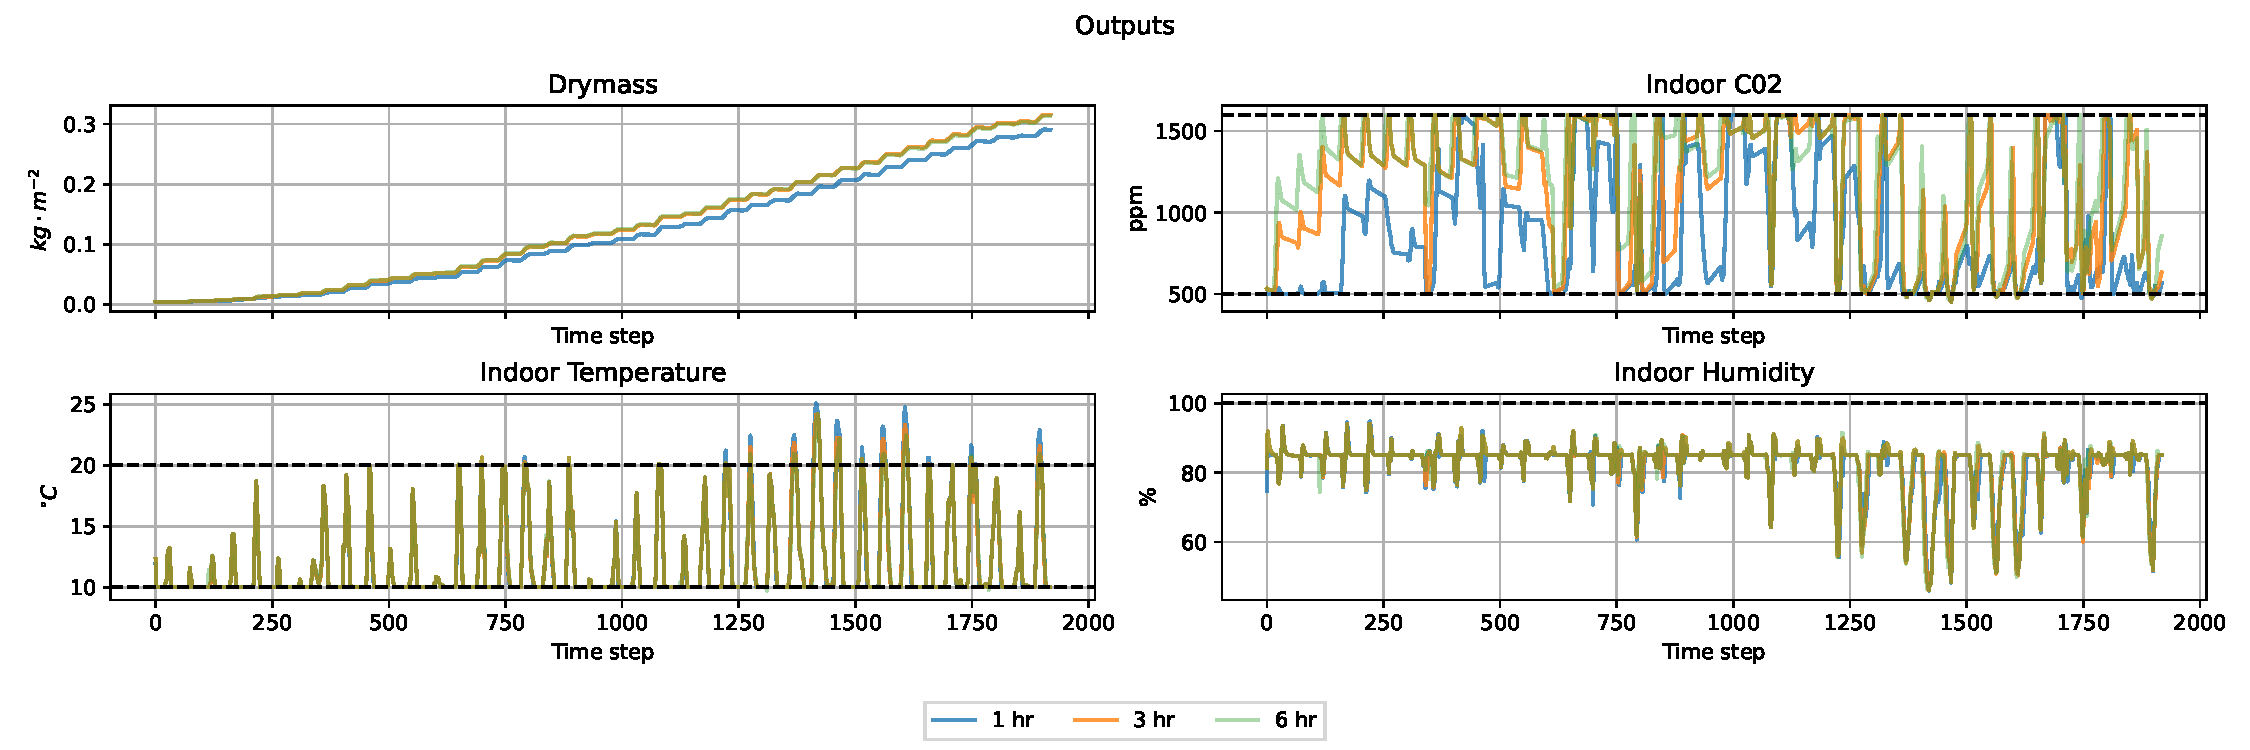
\includegraphics[width=\textwidth]{figures/mpc_outputs_time_series.eps}
	\caption{MPC 1hr and 5hr Time series of greenhouse outputs}
	\label{fig:mpc-timeseries-outputs}
\end{figure}

\begin{figure}[H]
	\centering
	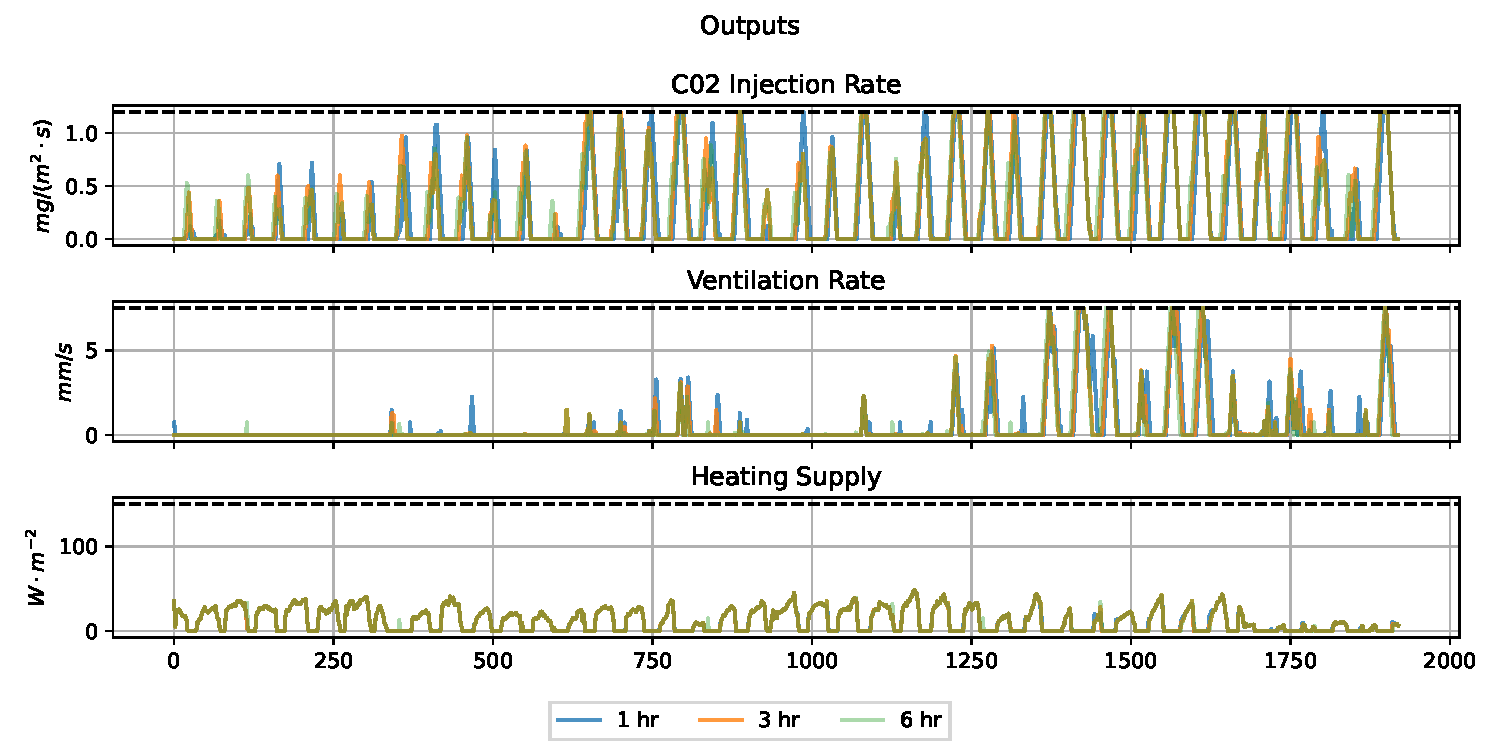
\includegraphics[width=\textwidth]{figures/mpc_inputs_times_series.eps}
	\caption{MPC 1hr and 5hr time series of controller inputs}
	\label{fig:mpc-timeseries-inputs}
\end{figure}

\autoref{fig:mpc-timeseries-outputs} and \autoref{fig:mpc-timeseries-inputs} displays the trajectories of the states and inputs of the best performing MPC controller (5hr prediction horizon) and the worst performing (1 hr). These bear similarities to those of the RL agents \autoref{fig:selected-policies-outputs} and \autoref{fig:selected-policies-inputs} respectively. It is noted that in both cases (RL and MPC), the better performing policies rapidly raises the indoor C02 levels at the beginning of the growing period by reducing ventilation and increasing C02 injection. However, the trajectories of other states and inputs, particularly the indoor temperature, humidity and heating, appear to be unchanged. Either the temperature does not play a vital role in plant growth or the prediction horizon is not long enough to see the effect of temperature at initial growth stages. However, it is clear that the MPC controller uses heating at night and the irradiance during the day to ensure that temperature constraints are met. These results are very similar to \cite{morcegoReinforcementLearningModel2023} and \cite{boersmaRobustSamplebasedModel2022} although difficult to compare quantitatively due to the difference in the optimization goal and MPC problem formulation.


\section{Stochastic Results}
For each stochastic level, $\delta = 5\%, \delta = 10\%, \delta = 20\%$, was analyzed with prediction horizons of 1, 3, and 5 hours. Additional prediction horizons were not considered due to limitations in simulation time. 


\section{Conclusion}
\emph{A brief conclusion of the work done and what will be carried over to the RL-MPC framework}